\documentclass[conference]{IEEEtran}
\usepackage{tikz}
\usepackage{xcolor}
\usepackage{amsmath,amssymb}
\usepackage{graphicx}

\usetikzlibrary{
    arrows.meta,
    positioning,
    fit,
    backgrounds,
    shapes.geometric,
    calc,
    decorations.pathreplacing
}

% Professional Color Palette (IEEE Standard compliant)
\definecolor{srcblue}{RGB}{220, 235, 252}
\definecolor{srcblueborder}{RGB}{41, 128, 185}
\definecolor{embteal}{RGB}{220, 248, 245}
\definecolor{embtealborder}{RGB}{22, 160, 133}
\definecolor{chromagray}{RGB}{240, 243, 244}
\definecolor{chromaborder}{RGB}{127, 140, 141}
\definecolor{reactgreen}{RGB}{232, 248, 235}
\definecolor{reactgreenborder}{RGB}{39, 174, 96}
\definecolor{toolamber}{RGB}{254, 249, 231}
\definecolor{toolamberborder}{RGB}{243, 156, 18}
\definecolor{dselorange}{RGB}{253, 237, 236}
\definecolor{dselorangeborder}{RGB}{231, 76, 60}
\definecolor{uiindigo}{RGB}{238, 238, 255}
\definecolor{uiindigoborder}{RGB}{102, 102, 204}

\begin{document}

\begin{figure*}[!t]
\centering
\resizebox{0.98\textwidth}{!}{%
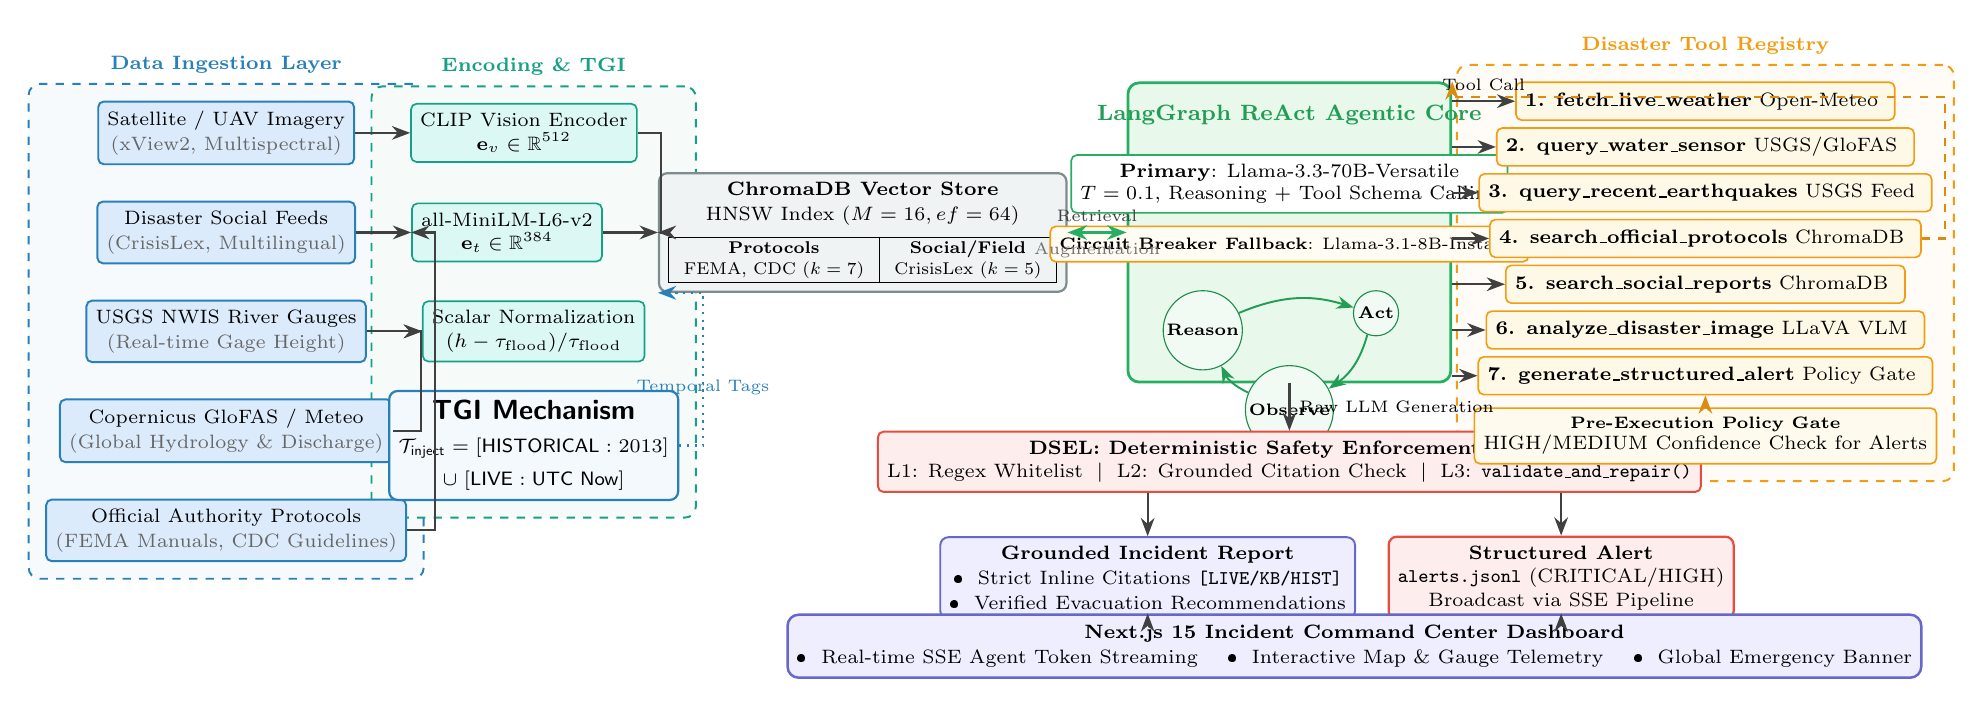
\begin{tikzpicture}[
    >=Stealth,
    node distance=0.45cm and 0.55cm,
    font=\sffamily,
    % Box styles
    srcbox/.style={
        draw=srcblueborder, fill=srcblue, rounded corners=2pt,
        align=center, minimum width=2.4cm, minimum height=0.62cm,
        font=\fontsize{7.5}{9}\selectfont, line width=0.7pt
    },
    embnode/.style={
        draw=embtealborder, fill=embteal, rounded corners=2pt,
        align=center, minimum width=2.3cm, minimum height=0.55cm,
        font=\fontsize{7}{8.5}\selectfont, line width=0.6pt
    },
    chromabox/.style={
        draw=chromaborder, fill=chromagray, rounded corners=3pt,
        align=center, minimum width=2.7cm, minimum height=0.9cm,
        font=\fontsize{7.5}{9}\selectfont, line width=0.8pt
    },
    reactbox/.style={
        draw=reactgreenborder, fill=reactgreen, rounded corners=4pt,
        align=center, minimum width=4.1cm, minimum height=3.8cm,
        font=\fontsize{8}{10}\selectfont, line width=1.0pt
    },
    toolnode/.style={
        draw=toolamberborder, fill=toolamber, rounded corners=2pt,
        align=left, minimum width=3.3cm, minimum height=0.48cm,
        font=\fontsize{6.8}{8}\selectfont, line width=0.6pt
    },
    dselnode/.style={
        draw=dselorangeborder, fill=dselorange, rounded corners=2pt,
        align=center, minimum width=3.4cm, minimum height=0.55cm,
        font=\fontsize{7}{8.5}\selectfont, line width=0.7pt
    },
    uibox/.style={
        draw=uiindigoborder, fill=uiindigo, rounded corners=3pt,
        align=center, minimum width=3.2cm, minimum height=0.6cm,
        font=\fontsize{7.5}{9}\selectfont, line width=0.7pt
    },
    % Group container styles
    groupbox/.style={
        draw=#1, dashed, rounded corners=4pt, fill=#1!4,
        inner sep=6pt, line width=0.7pt
    },
    % Arrow styles
    dataflow/.style={->, line width=0.8pt, draw=black!75},
    fbflow/.style={<->, line width=0.9pt, draw=reactgreenborder},
    alertflow/.style={->, line width=0.9pt, draw=dselorangeborder, dashed},
    tgifflow/.style={->, line width=0.8pt, draw=srcblueborder, dotted}
]

% =========================================================================
% LAYER 1: MULTIMODAL INGESTION DATA SOURCES (Left Column)
% =========================================================================
\node[srcbox] (src_sat) {Satellite / UAV Imagery\\{\scriptsize\color{black!60}(xView2, Multispectral)}};
\node[srcbox, below=of src_sat] (src_soc) {Disaster Social Feeds\\{\scriptsize\color{black!60}(CrisisLex, Multilingual)}};
\node[srcbox, below=of src_soc] (src_wat) {USGS NWIS River Gauges\\{\scriptsize\color{black!60}(Real-time Gage Height)}};
\node[srcbox, below=of src_wat] (src_glo) {Copernicus GloFAS / Meteo\\{\scriptsize\color{black!60}(Global Hydrology \& Discharge)}};
\node[srcbox, below=of src_glo] (src_fema) {Official Authority Protocols\\{\scriptsize\color{black!60}(FEMA Manuals, CDC Guidelines)}};

% =========================================================================
% LAYER 2: EMBEDDING & TEMPORAL GROUNDING INJECTION (TGI)
% =========================================================================
\node[embnode, right=0.7cm of src_sat] (emb_clip) {CLIP Vision Encoder\\{\scriptsize $\mathbf{e}_v \in \mathbb{R}^{512}$}};
\node[embnode, right=0.7cm of src_soc] (emb_text) {all-MiniLM-L6-v2\\{\scriptsize $\mathbf{e}_t \in \mathbb{R}^{384}$}};
\node[embnode, right=0.7cm of src_wat] (emb_sensor) {Scalar Normalization\\{\scriptsize $(h - \tau_{\text{flood}})/\tau_{\text{flood}}$}};

% TGI Injection Box
\node[draw=srcblueborder, fill=srcblue!30, rounded corners=3pt, line width=0.8pt,
      minimum width=2.6cm, minimum height=1.1cm, align=center,
      below=0.35cm of emb_sensor] (tgi_box) {
      \textbf{TGI Mechanism}\\
      \scriptsize $\mathcal{T}_{\text{inject}} = [\text{HISTORICAL}: 2013]$\\
      \scriptsize $\cup\; [\text{LIVE}: \text{UTC Now}]$
};

% =========================================================================
% LAYER 3: VECTOR STORE & KNOWLEDGE BASE
% =========================================================================
\node[chromabox, right=0.7cm of emb_text] (chroma_db) {
    \textbf{ChromaDB Vector Store}\\
    \scriptsize HNSW Index ($M=16, ef=64$)\\[3pt]
    \scalebox{0.88}{%
    \begin{tabular}{|c|c|}
    \hline
    \textbf{Protocols} & \textbf{Social/Field} \\
    FEMA, CDC ($k=7$) & CrisisLex ($k=5$) \\
    \hline
    \end{tabular}}
};

% =========================================================================
% LAYER 4: AGENTIC CORE (LangGraph ReAct Loop)
% =========================================================================
\node[reactbox, right=0.75cm of chroma_db] (agent_core) {};

% Inner nodes within Agent Box
\node[anchor=north, align=center, font=\bfseries\fontsize{8.5}{10}\selectfont, text=reactgreenborder!90!black, yshift=-5pt] 
    at (agent_core.north) (agent_header) {LangGraph ReAct Agentic Core};

\node[draw=reactgreenborder, fill=white, rounded corners=2pt, line width=0.6pt,
      minimum width=3.6cm, minimum height=0.6cm, align=center,
      below=0.25cm of agent_header, font=\fontsize{7}{8}\selectfont] (llm_primary) {
      \textbf{Primary}: Llama-3.3-70B-Versatile\\
      {\scriptsize $T=0.1$, Reasoning + Tool Schema Calling}
};

\node[draw=toolamberborder, fill=toolamber!50, rounded corners=2pt, line width=0.6pt,
      minimum width=3.6cm, minimum height=0.45cm, align=center,
      below=0.15cm of llm_primary, font=\fontsize{6.5}{7.5}\selectfont] (circuit_breaker) {
      \textbf{Circuit Breaker Fallback}: Llama-3.1-8B-Instant
};

% Circular ReAct State Machine inside Agent Core
\node[circle, draw=reactgreenborder!80!black, fill=reactgreen!60, inner sep=1pt,
      below=0.35cm of circuit_breaker, xshift=-1.1cm, font=\fontsize{6.5}{7}\selectfont\bfseries] (s_reason) {Reason};
\node[circle, draw=reactgreenborder!80!black, fill=reactgreen!60, inner sep=1pt,
      below=0.35cm of circuit_breaker, xshift=1.1cm, font=\fontsize{6.5}{7}\selectfont\bfseries] (s_act) {Act};
\node[circle, draw=reactgreenborder!80!black, fill=reactgreen!60, inner sep=1pt,
      below=0.55cm of $(s_reason)!0.5!(s_act)$, font=\fontsize{6.5}{7}\selectfont\bfseries] (s_obs) {Observe};

\draw[->, line width=0.7pt, draw=reactgreenborder!90!black] (s_reason) to[bend left=20] (s_act);
\draw[->, line width=0.7pt, draw=reactgreenborder!90!black] (s_act) to[bend left=20] (s_obs);
\draw[->, line width=0.7pt, draw=reactgreenborder!90!black] (s_obs) to[bend left=20] (s_reason);

\node[below=0.08cm of s_obs, font=\fontsize{6.2}{7}\selectfont, text=black!65] {Multi-turn State \& SQLite Memory};

% =========================================================================
% LAYER 5: TOOL EXECUTION REGISTRY (Right Stack)
% =========================================================================
\node[toolnode, right=0.8cm of agent_core.north east, anchor=north west] (t1) {
    \textbf{1. fetch\_live\_weather} \hfill {\scriptsize Open-Meteo}
};
\node[toolnode, below=0.08cm of t1] (t2) {
    \textbf{2. query\_water\_sensor} \hfill {\scriptsize USGS/GloFAS}
};
\node[toolnode, below=0.08cm of t2] (t3) {
    \textbf{3. query\_recent\_earthquakes} \hfill {\scriptsize USGS Feed}
};
\node[toolnode, below=0.08cm of t3] (t4) {
    \textbf{4. search\_official\_protocols} \hfill {\scriptsize ChromaDB}
};
\node[toolnode, below=0.08cm of t4] (t5) {
    \textbf{5. search\_social\_reports} \hfill {\scriptsize ChromaDB}
};
\node[toolnode, below=0.08cm of t5] (t6) {
    \textbf{6. analyze\_disaster\_image} \hfill {\scriptsize LLaVA VLM}
};
\node[toolnode, below=0.08cm of t6] (t7) {
    \textbf{7. generate\_structured\_alert} \hfill {\scriptsize Policy Gate}
};

% =========================================================================
% LAYER 6: DETERMINISTIC SAFETY ENFORCEMENT LAYER (DSEL)
% =========================================================================
\node[dselnode, below=0.6cm of agent_core.south] (dsel_box) {
    \textbf{DSEL: Deterministic Safety Enforcement Layer}\\
    \scriptsize L1: Regex Whitelist \;\textbar\; L2: Grounded Citation Check \;\textbar\; L3: \texttt{validate\_and\_repair()}
};

% Policy Gate (Pre-execution)
\node[draw=toolamberborder, fill=toolamber!70, rounded corners=2pt, line width=0.6pt,
      minimum width=3.3cm, minimum height=0.45cm, align=center,
      below=0.15cm of t7, font=\fontsize{6.5}{7.5}\selectfont] (policy_engine) {
      \textbf{Pre-Execution Policy Gate}\\
      {\scriptsize HIGH/MEDIUM Confidence Check for Alerts}
};

% =========================================================================
% LAYER 7: GROUNDED OPERATIONAL OUTPUTS
% =========================================================================
\node[uibox, below=0.55cm of dsel_box, xshift=-1.8cm] (out_report) {
    \textbf{Grounded Incident Report}\\
    \scriptsize \textbullet\; Strict Inline Citations \texttt{[LIVE/KB/HIST]}\\
    \scriptsize \textbullet\; Verified Evacuation Recommendations
};

\node[draw=dselorangeborder, fill=dselorange, rounded corners=3pt, line width=0.8pt,
      minimum width=2.8cm, minimum height=0.6cm, align=center,
      right=0.4cm of out_report, font=\fontsize{7}{8.5}\selectfont] (out_alert) {
    \textbf{Structured Alert}\\
    \scriptsize \texttt{alerts.jsonl} (CRITICAL/HIGH)\\
    \scriptsize Broadcast via SSE Pipeline
};

% =========================================================================
% LAYER 8: OPERATOR INTERACTION FRONTEND
% =========================================================================
\node[draw=uiindigoborder, fill=uiindigo, rounded corners=4pt, line width=0.9pt,
      minimum width=8.5cm, minimum height=0.8cm, align=center,
      below=0.45cm of $(out_report)!0.5!(out_alert)$, font=\fontsize{7.5}{9}\selectfont] (frontend) {
    \textbf{Next.js 15 Incident Command Center Dashboard}\\
    \scriptsize \textbullet\; Real-time SSE Agent Token Streaming \quad
    \textbullet\; Interactive Map \& Gauge Telemetry \quad
    \textbullet\; Global Emergency Banner
};

% =========================================================================
% CONNECTIONS AND ARROWS
% =========================================================================
% Sources to Embeddings
\draw[dataflow] (src_sat) -- (emb_clip);
\draw[dataflow] (src_soc) -- (emb_text);
\draw[dataflow] (src_wat) -- (emb_sensor);
\draw[dataflow] (src_glo.east) -- ++(0.35,0) |- (emb_sensor.west);
\draw[dataflow] (src_fema.east) -- ++(0.35,0) |- (emb_text.west);

% Embeddings to ChromaDB
\draw[dataflow] (emb_clip.east) -- ++(0.3,0) |- (chroma_db.west);
\draw[dataflow] (emb_text) -- (chroma_db);

% TGI into ChromaDB metadata
\draw[tgifflow] (tgi_box.east) -- ++(0.3,0) |- node[near start, below, font=\fontsize{6}{7}\selectfont, text=srcblueborder] {Temporal Tags} (chroma_db.south west);

% ChromaDB to Agent (Multimodal retrieval)
\draw[fbflow] (chroma_db) -- node[midway, above, font=\fontsize{6.5}{7.5}\selectfont, text=black!75] {Retrieval}
                            node[midway, below, font=\fontsize{6.5}{7.5}\selectfont, text=black!55] {Augmentation} (agent_core.west);

% Agent to Tools
\draw[dataflow] (agent_core.east |- t1) -- node[above, font=\fontsize{6}{7}\selectfont] {Tool Call} (t1.west);
\draw[dataflow] (agent_core.east |- t2) -- (t2.west);
\draw[dataflow] (agent_core.east |- t3) -- (t3.west);
\draw[dataflow] (agent_core.east |- t4) -- (t4.west);
\draw[dataflow] (agent_core.east |- t5) -- (t5.west);
\draw[dataflow] (agent_core.east |- t6) -- (t6.west);
\draw[dataflow] (agent_core.east |- t7) -- (t7.west);

% Tools back to Agent (Observation)
\draw[dataflow, dashed, draw=toolamberborder!90!black] (t4.east) -- ++(0.3,0) -- ++(0,1.8) -| (agent_core.north east);

% Policy Engine to Alert Tool
\draw[dataflow, draw=toolamberborder!90!black] (policy_engine) -- (t7);

% Agent to DSEL
\draw[dataflow] (agent_core.south) -- node[midway, right, font=\fontsize{6.5}{7.5}\selectfont] {Raw LLM Generation} (dsel_box.north);

% DSEL to Outputs
\draw[dataflow] (dsel_box.south -| out_report.north) -- (out_report.north);
\draw[dataflow] (dsel_box.south -| out_alert.north) -- (out_alert.north);

% Outputs to Frontend
\draw[dataflow] (out_report.south) -- (out_report.south |- frontend.north);
\draw[dataflow] (out_alert.south) -- (out_alert.south |- frontend.north);

% Background Groups for visual hierarchy
\begin{scope}[on background layer]
    \node[groupbox=srcblueborder, fit=(src_sat) (src_fema),
          label={[font=\fontsize{7}{8}\selectfont\bfseries, text=srcblueborder]above:Data Ingestion Layer}] {};
    \node[groupbox=embtealborder, fit=(emb_clip) (tgi_box),
          label={[font=\fontsize{7}{8}\selectfont\bfseries, text=embtealborder]above:Encoding \& TGI}] {};
    \node[groupbox=toolamberborder, fit=(t1) (policy_engine),
          label={[font=\fontsize{7}{8}\selectfont\bfseries, text=toolamberborder]above:Disaster Tool Registry}] {};
\end{scope}

\end{tikzpicture}
}
\caption{System Architecture of the Multimodal Agentic Retrieval-Augmented Generation (RAG) Disaster Intelligence Framework. The pipeline orchestrates multimodal ingestion (satellite, social, hydrological, protocol feeds), applies Temporal Grounding Injection (TGI), maintains an HNSW-indexed vector store, and drives an autonomous LangGraph ReAct agent loop. Generated actions pass through a Deterministic Safety Enforcement Layer (DSEL) and pre-execution policy gate prior to operator dissemination.}
\label{fig:system_architecture}
\end{figure*}

\end{document}

